\documentclass{ximera}[font=12pt]

% Terminal command to remove xmcss files, must be in /workspaces/BlueFish
% find . -name "*.xmcss" -type f -delete

\title{Adding Integers: Introduction}   % Use xmlatex all -s to compile when SERVE refuses to work.
\author{Kelly Stady}
\license{CC: 0}         % replace with an appropriate license, or set it in xmPreamble

\begin{document}  


\begin{abstract}

\end{abstract}


\maketitle
\label{xim:AddIntroActivity}


\section*{The Set of Integers}

In this lesson, you will learn how to add numbers that belong to the set of integers.  The set of \textbf{integers} consists of the whole numbers along with the negative counting numbers.

\begin{description}[itemsep=1ex]  % an ex is the height of a lowercase x
    \item[\textbf{Counting Numbers}] $\{ 1, 2, 3, \ldots \}$
    \item[\textbf{Whole Numbers}] $\{0, 1, 2, 3, \ldots \}$
    \item[\textbf{Integers}] $\{ \ldots, -5, -4, -3, -2, -1, 0, 1, 2, 3, 4, 5, \ldots \}$
\end{description}

~ \\[2em]


\begin{tikzpicture}[scale=0.4]
    % Frames (the outer "rims")
    \draw[line width=2pt, fill=blue!5] (0,0) circle (0.9);
    \draw[line width=2pt, fill=blue!5] (2.4,0) circle (0.9);

    % The "Coke Bottle" Lens Effect (thin gray rings on the light background)
    %\foreach \r in {0.7, 0.5, 0.3} {
       % \draw[gray!40, thin] (0,0) circle (\r);
       % \draw[gray!40, thin] (2.4,0) circle (\r);
    %}

    % Reflection glints (adds a "glass" feel)
    \fill[white, opacity=0.8] (-0.4,0.4) circle (0.15);
    \fill[white, opacity=0.8] (2.0,0.4) circle (0.15);

    % Bridge
    \draw[line width=2pt] (0.9,0.1) arc (150:30:0.35);

    % Temples (Arms)
    \draw[line width=2pt] (-0.9,0.3) -- (-1.8,0.7);
    \draw[line width=2pt] (3.3,0.3) -- (4.2,0.7);
\end{tikzpicture}

\section*{Extra Insight}

\normalsize
Although negative numbers were understood in China more than 2000 years ago and later in India, they were not immediately accepted in Europe.
For many centuries, European mathematicians were uncomfortable with the idea of numbers less than zero and sometimes referred to them  as ``false" or
``absurd" numbers.  However, during the 16th and 17th centuries, as algebra and calculus developed, the importance of negative numbers became undeniable.
Today, negative numbers are an essential part of mathematics and are commonly used to represent quantities such as losses, debts, temperatures below zero and
elevations below sea level.

\section*{Adding Integers}

To understand how to add integers, we will begin by using the Chinese Red-Black Rule and then a number line to visualize addition.  Then we will use the concepts of assets and debts to understand addition in a real-world context.  These approaches will lead us to two rules: one for adding numbers with the same sign and another for adding numbers with different signs.

\subsection*{The Red-Black Rule}

Negative numbers were first used systematically in ancient China. In \emph{The Nine Chapters on the Mathematical Art} (written between about 200 BC and 100 AD), Chinese mathematicians used counting rods to represent numbers.  Red rods were used for positive numbers and black rods for negative numbers.  For example, the number 3 was
represented by three red rods and the number $-2$ was represented by two black rods.  These rods were used as a calculator of sorts for financial transactions involving profits and losses and to solve simple equations.  The Red-Black Rule is described below.

\begin{enumerate}[itemsep=2ex]
\item A red rod represents $1$ and a black rod $-1.$

\item To find the total of profits (red) and losses (black), begin by placing rods on a board to represent each number.

\item Since a profit and an equal loss result in 0, gather all pairs of red and black rods and remove them.

\item The total is what remains.
\end{enumerate}


Since red and black can be difficult for some people to distinguish, we will use \textcolor{orange!85!black}{\textbf{orange rods}} to represent \textcolor{orange!85!black}{\textbf{positive numbers}} and \textcolor{blue!70!black}{\textbf{blue rods}} to represent \textcolor{blue!70!black}{\textbf{negative numbers}}.
We will now refer to this rule as the Orange-Blue Rule.


\begin{example} To find the sum $-5+3,$ begin with \textcolor{blue!70!black}{\textbf{five blue rods}} to represent the number $-5$ and \textcolor{orange!85!black}{\textbf{three orange rods}} to represent the number $3.$  Next remove all pairs of orange and blue rods.  Since two blue rods remain, the answer is $-2.$

~ \\[4em] % Puts some vertical space- yippie!!!******************************************************************
\begin{tikzpicture}[scale=0.75, font=\sffamily]
     
% Define Accessible Colors
\colorlet{posColor}{orange!85!black}  % 85% orange, 15% black
\colorlet{negColor}{blue!70!black}

% --- SECTION 1: THE SETUP ---
    \begin{scope}[shift={(-5,0)}]
        \node[font=\bfseries\small, black!80, anchor=west] at (-0.3, 2.4) {Setup};

        % Value: -5
        \node[font=\bfseries, negColor, anchor=east] at (-0.2, 1.0) {$-5$};
        \foreach \x in {0, 0.4, 0.8, 1.2, 1.6} {
            \draw[line width=2.5pt, negColor, cap=round] (\x, 0.5) -- (\x, 1.5);
            %\node[negColor, font=\tiny\bfseries] at (\x, 1.7) {$-$};  % - Signs above Bars
        }

        % Value: +3
        \node[font=\bfseries, posColor, anchor=east] at (-0.2, -0.3) {$3$};
        \foreach \x in {0, 0.4, 0.8} {
            \draw[line width=2.5pt, posColor, cap=round] (\x, -0.8) -- (\x, 0.2);
            %\node[posColor, font=\tiny\bfseries] at (\x, -1.0) {$+$}; % + Signs above Bars
        }
    \end{scope}

    % --- SECTION 2: Remove Pairs ---
    \begin{scope}[shift={(0,0)}]
        \node[font=\bfseries\small] at (0.75, 2.4) {Remove Pairs};

        % The 3 Pairs that will cancel
        \foreach \x in {0, 0.4, 0.8} {
            \draw[line width=2.5pt, negColor, cap=round] (\x, 0.5) -- (\x, 1.5);
            \draw[line width=2.5pt, posColor, cap=round] (\x, -0.8) -- (\x, 0.2);
        }

        % CANCELLATION BOX
        \draw[dashed, black!40, line width=1pt, rounded corners=5pt] (-0.25, -1.1) rectangle (1.05, 1.9);

        % THE LEFTOVER BARS
        \foreach \x in {1.5, 1.9} {
            \draw[line width=2.5pt, negColor, cap=round] (\x, 0.5) -- (\x, 1.5);
            %\node[negColor, font=\tiny\bfseries] at (\x, 1.7) {$-$};
        }

        % Transition arrow
        \draw[->, ultra thick, glaucous] (3.2, 0.3) -- (4.2, 0.3);
    \end{scope}

    % --- SECTION 3: THE RESULT ---
    \begin{scope}[shift={(5.5,0)}]
        \node[font=\bfseries\small] at (0.2, 2.4) {Result};

        % Only the 2 surviving Negative Rods
        \foreach \x in {0, 0.4} {
            \draw[line width=3pt, negColor, cap=round] (\x, 0.3) -- (\x, 1.3);
            %\node[negColor, font=\tiny\bfseries] at (\x, 1.5) {$-$};
        }

        % The Result Label
        \node[anchor=north, negColor, font=\bfseries] at (0.1, -0.2) {$-2$};
    \end{scope}

    % Bottom equation
    \node[anchor=north, black!80, font=\bfseries] at (-5, -2) {$-5 + 3 = -2$};

\end{tikzpicture}

\end{example}

~ \\[0.5em]

\begin{example}  To find the sum $-4+(-3),$ begin with \textcolor{blue!70!black}{\textbf{four blue rods}} to represent the number $-4$ and \textcolor{blue!70!black}{\textbf{three blue rods}} to represent the number $-3.$  Since there are no orange-blue pairs to remove, 7 blue rods remain, so the answer is $-7.$


    ~ \\[4em] % Forces space in html
\begin{tikzpicture}[scale=0.75, font=\sffamily]
% Define Accessible Colors
\colorlet{posColor}{orange!80!black}
\colorlet{negColor}{blue!70!black}

% --- SECTION 1: THE SETUP (Lined up vertically) ---
    \begin{scope}[shift={(-6.5,0)}]
        \node[font=\bfseries\small, black, anchor=west] at (-0.3, 2.2) {Setup};

        % Value: -4 (4 Blue vertical rods)
        \node[font=\bfseries, negColor, anchor=east] at (-0.2, 1.0) {$-4$};
        \foreach \x in {0, 0.4, 0.8, 1.2}
            \draw[line width=2.5pt, negColor, cap=round] (\x, 0.5) -- (\x, 1.5);

        % Value: -3 (3 Blue vertical rods)
        \node[font=\bfseries, blue!80!black, anchor=east] at (-0.2, -0.3) {$-3$};
        \foreach \x in {0, 0.4, 0.8}
            \draw[line width=2.5pt, negColor, cap=round] (\x, -0.8) -- (\x, 0.2);
    \end{scope}

    % --- SECTION 2: Combine Rods (No Pairs to Remove)
    \begin{scope}[shift={(0,0)}]
        \node[font=\bfseries\small] at (0.75, 2.2) {Remove Pairs};

        % All rods are blue, so they all stay
        \foreach \x in {0, 0.4, 0.8, 1.2}
            \draw[line width=2.5pt, negColor, cap=round] (\x, 0.5) -- (\x, 1.5);

        \foreach \x in {0, 0.4, 0.8}
            \draw[line width=2.5pt, negColor, cap=round] (\x, -0.8) -- (\x, 0.2);

        \node[darkraspberry, font=\bfseries\small, align=center] at (0.9, -1.35) {No Pairs to Remove!};

        % Transition arrow
        \draw[->, ultra thick, glaucous] (2.2, 0.3) -- (3.2, 0.3);
    \end{scope}

    % --- SECTION 3: THE RESULT ---
    \begin{scope}[shift={(4.5,0)}]
        \node[font=\bfseries\small] at (1.2, 2.2) {Result};

        % All 7 surviving Negative Rods
        \foreach \x in {0, 0.4, 0.8, 1.2, 1.6, 2.0, 2.4}
            \draw[line width=2.5pt, blue!80!black, cap=round] (\x, 0.3) -- (\x, 1.3);

        % The Result Label
        \node[anchor=north, negColor, font=\bfseries] at (1.2, -0.2) {$-7$};
        \node[anchor=north, black, font=\bfseries] at (-10.1, -2) {$-4 + (-3) = -7$};
    \end{scope}

\end{tikzpicture}

\end{example}

~ \\[1em]

\begin{problem}
Use the Blue-Orange Rule to find the sum $-2+6.$  The problem has been setup for you below.

~ \\[3em]  %Forces vertical space

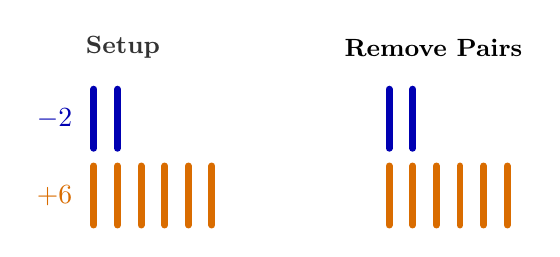
\begin{tikzpicture}[scale=0.75, font=\sffamily]

% Define Accessible Colors
\colorlet{posColor}{orange!85!black}
\colorlet{negColor}{blue!70!black}

% --- SECTION 1: THE SETUP (Lined up vertically) ---

    \begin{scope}[shift={(-5,0)}]
    \node[font=\bfseries\small, black!80, anchor=west] at (-0.3, 2.2) {Setup};

% Value: -2 (2 Blue vertical rods)
    \node[font=\bfseries, negColor, anchor=east] at (-0.2, 1.0) {$-2$};
    \foreach \x in {0, 0.4}
    \draw[line width=2.5pt, negColor, cap=round] (\x, 0.5) -- (\x, 1.5);

% Value: +6 (6 Orange vertical rods)
    \node[font=\bfseries, posColor, anchor=east] at (-0.2, -0.3) {$+6$};
    \foreach \x in {0, 0.4, 0.8, 1.2, 1.6, 2.0}
    \draw[line width=2.5pt, posColor, cap=round] (\x, -0.8) -- (\x, 0.2);
    \end{scope}

% --- SECTION 2: Remove Pairs ---
    \begin{scope}[shift={(0,0)}]
    \node[font=\bfseries\small] at (0.75, 2.2) {Remove Pairs};

% The 2 Pairs that will cancel (Inside the box)
    \foreach \x in {0, 0.4} {
    \draw[line width=2.5pt, negColor, cap=round] (\x, 0.5) -- (\x, 1.5); % Blue
    \draw[line width=2.5pt, posColor, cap=round] (\x, -0.8) -- (\x, 0.2); % Orange
    }

% THE LEFTOVER BARS (4 orange rods remain)
    \foreach \x in {0.8, 1.2, 1.6, 2.0}
    \draw[line width=2.5pt, posColor, cap=round] (\x, -0.8) -- (\x, 0.2);

    \end{scope}

\end{tikzpicture}

$-2 + 6 \begin{prompt} =  \answer{4} \end{prompt}$

\end{problem}


~ \\[12pt]  % Vertical Space :)
The use of colors in the Orange-Blue Rule is not necessary. Below is the first example redone using plus signs ($+$) for 
positive numbers and minus signs ($-$) signs for negative numbers.  You can also use things like rocks and sticks or
pennies and dimes---the sky's the limit!  Try modifying the rule, using your own way to represent positive and negative 
numbers.  Be creative!


%Trying to get vertical spacing!  Seeing what works in the html


%\mbox{} \\  Too much spacing, but works!

%\paragraph{Example III}

\begin{example} To find the sum $-5+3,$ begin with \textbf{five minus signs} $(-)$ to represent the number $-5$ and 
    \textbf{three plus signs} $(+)$ to represent the number $3.$  Next remove all $+$ $-$ pairs.  
    Since two minus ($-$) signs remain, the answer is $-2.$  

    ~ \\[3em] %Vertical spacing

\begin{tikzpicture}[scale=0.75, font=\sffamily]
% --- SECTION 1: THE SETUP (Lined up vertically) ---
    \begin{scope}[shift={(-5,0)}]
        \node[font=\bfseries\small, black!80, anchor=west] at (-0.5, 2.2) {Setup};

        % Value: -5 (Increased spacing from 0.4 to 0.7)
        \node[font=\bfseries, black, anchor=east] at (-0.3, 1.0) {$-5$};
        \foreach \x in {0, 0.7, 1.4, 2.1, 2.8}
            \node[black, font=\huge] at (\x, 1.0) {$-$};

        % Value: +3 (Increased spacing from 0.4 to 0.7)
        \node[font=\bfseries, black, anchor=east] at (-0.3, -0.3) {$3$};
        \foreach \x in {0, 0.7, 1.4}
            \node[black, font=\bfseries] at (\x, -0.3) {+};
    \end{scope}

    % --- SECTION 2: Remove Pairs
    \begin{scope}[shift={(0,0)}]
        \node[font=\bfseries\small] at (1.3, 2.2) {Remove Pairs};

        % The 3 Pairs that will cancel (Inside the box)
        \foreach \x in {0, 0.7, 1.4} {
            \node[black, font=\huge] at (\x, 1.0) {$-$}; % Negative
            \node[black, font=\bfseries] at (\x, -0.3) {+}; % Positive
        }

        % CANCELLATION BOX (Adjusted width for wider spacing)
        \draw[dashed, black!80, line width=1.1pt, rounded corners=5pt] (-0.5, -1.0) rectangle (1.9, 1.7);

        % THE LEFTOVER -s
        \foreach \x in {2.4, 3.1}
            \node[black, font=\huge] at (\x, 1.0) {$-$};

        % Transition arrow
        \draw[->, ultra thick, glaucous] (4.5, 0.3) -- (5.5, 0.3);

    \end{scope}

    % --- SECTION 3: THE RESULT ---
    \begin{scope}[shift={(7.5,0)}] % Shifted Result section right to accommodate wider previous sections
        \node[font=\bfseries\small] at (0.35, 2.2) {Result};

        % Only the 2 surviving - signs
        \foreach \x in {0, 0.7}
            \node[black, font=\huge] at (\x, 0.8) {$-$};

        % The Result Label
        \node[anchor=north, black, font=\bfseries] at (0.35, -0.2) {$-2$};
        \node[anchor=north, black, font=\bfseries] at (-12.1, -2) {$-5 +3 = -2 $};

    \end{scope}

\end{tikzpicture}

\end{example}

~ \\[12pt]

Although this modified rule isn't overly creative, it makes the answer quite clear.


\end{document}